\chapter{Análise Bibliográfica sobre Mineração de Dados na área de Medicina, por Vinícius Caixeta de Souza}

\section{Planejamento do estudo}

A mineração de dados é comumente associada ao mercado devido a análise de produtos que o consumidor queira comprar com base nos seus dados de compras, porém existem várias outras áreas que se beneficiam da mineração de dados como medicina para prever o número de pacientes com cada categoria e detecção de fraudes.

Este estudo fará a análise bibliográfica sobre a mineração de dados em particular na área de medicina para tentar responder as seguintes perguntas:

\begin{itemize}
    \item Quais são os autores que mais produzem artigos relacionados a mineração de dados na área de medicina?
    \item O surgimento do coronavírus deu um impulso na produção de artigos?
    \item Quais são os principais padrões que a mineração de dados busca explorar?
\end{itemize}

\subsection{Uso do Bibliometrix e Biblioshiny}
Neste estudo serão utilizados a ferramenta e o workflow Bibliometrix e Biblioshiny da linguagem R para poder visualizar dados e gráficos relacionados a lista de base obtida.

\section{Coleta de Dados}
A coleta de dados foi feita no dia 04 de Fevereiro de 2022 a partir do Web Of Science por meio do Portal de Periódicos da CAPES, disponibilizado graças ao acesso CAFe. Para realizar a busca utilizou-se a query ilustrada a seguir:

\lstinputlisting[numbers=left,basicstyle=\normalsize\ttfamily,caption={\query\  de busca sobre mineração de dados na área de medicina.},label=query20220204-vinis-caixe]
{experiments/vinis-caixe/PesqBibliogr/MineracaoDados/WoS-20220204/query.txt}

\subsection{Explicação para os termos de busca usados}
Data e Mining foram usados para recuperar artigos relacionados a mineração de dados, health care, medicine e medical utilizados para obter artigos sobre a área de medicina e a palavra patient foi usada para obter artigos que possuam dados de pacientes em específico. No decorrer da análise poderá haver um refinamento dessa \query\.

O resultado foi uma lista com 7367 registros, ela foi obtida usando a opção exportar arquivo de texto sem formatação, contendo todas as seleções possíveis no Web of Science. Os registros foram recuperados em oito blocos de até 1.000 registros por vez (1-1000, 1001-2000, 2001-3000, ..., 7001-7367).

\section{Análise dos dados}

\subsection{Filtragem de registros}

O Biblioshiny possui a função de filtrar registros na lista de base sobre o tipo de documento, como a análise será somente de artigos científicos será aplicado esse filtro para tirar todos os outros documentos. Dentre os 7367 registros iniciais somente 4967 eram artigos.

\subsection{Análise descritiva do \dataset\ }

As principais informações sobre a lista são:

\begin{description}
    \item [\textit{Timespan}] Os artigos com publicação mais antigo na lista são de 1991, até 2022. Logo, não foram encontrados artigos entre 1945 até 1990.
    \item [\textit{Sources (Journals, Books, etc)}] Os artigos foram publicados por 1786 fontes de informação. Então, em média, cada \textit{scientific journal} publicou $4.967/1.786=2,8$ artigos.
    \item [\textit{Average years from publication}] O tempo de publicação dos registros no \dataset\ é, em média, 5,7 anos.
    \item [\textit{Average citations per documents}] A média de citações por documento é 17,34.
    \item [\textit{Average citations per year per doc}] Cada artigo foi citado em média 2,262 vezes por ano.
    \item [\textit{References}] O \dataset\  contém 161.118 referências citadas.
    \item [\textit{Keywords Plus (ID)}] Foram encontradas 9.547 distintas palavras-chave.
    \item [\textit{Author's Keywords (DE)}] Foram encontradas 10.907 distintas palavras-chave indicadas pelos autores.
    \item [\textit{Authors}] Foram encontrados 27.072 autores responsáveis pelos artigos.
    \item [\textit{Author Appearances}] Os 27.072 distintos  autores foram encontrados 39.908 vezes, como autores de artigos.
    \item [\textit{Authors of single-authored documents}] Somente 100 autores publicaram documentos por conta própria.
    \item [\textit{Authors of multi-authored documents}] 26.972 autores publicaram artigos com co-autoria.
    \item [\textit{Single-authored documents}] Somente 110 artigos foram publicados por um único autor.
    \item [\textit{Documents per Author}] A média de documentos que cada autor publicou é de 0,183.
    \item [\textit{Authors per Document}] Cada artigo foi publicado por, em média, 5,45 autores.
    \item [\textit{Co-Authors per Documents}] Cada artigo tem, em média, 8,03 co-autores.
    \item [\textit{Collaboration Index}] O índice de colaboração do \dataset\ é 5,55
\end{description}

\subsection{Evolução da Produção Científica}

\begin{figure}
    \centering
    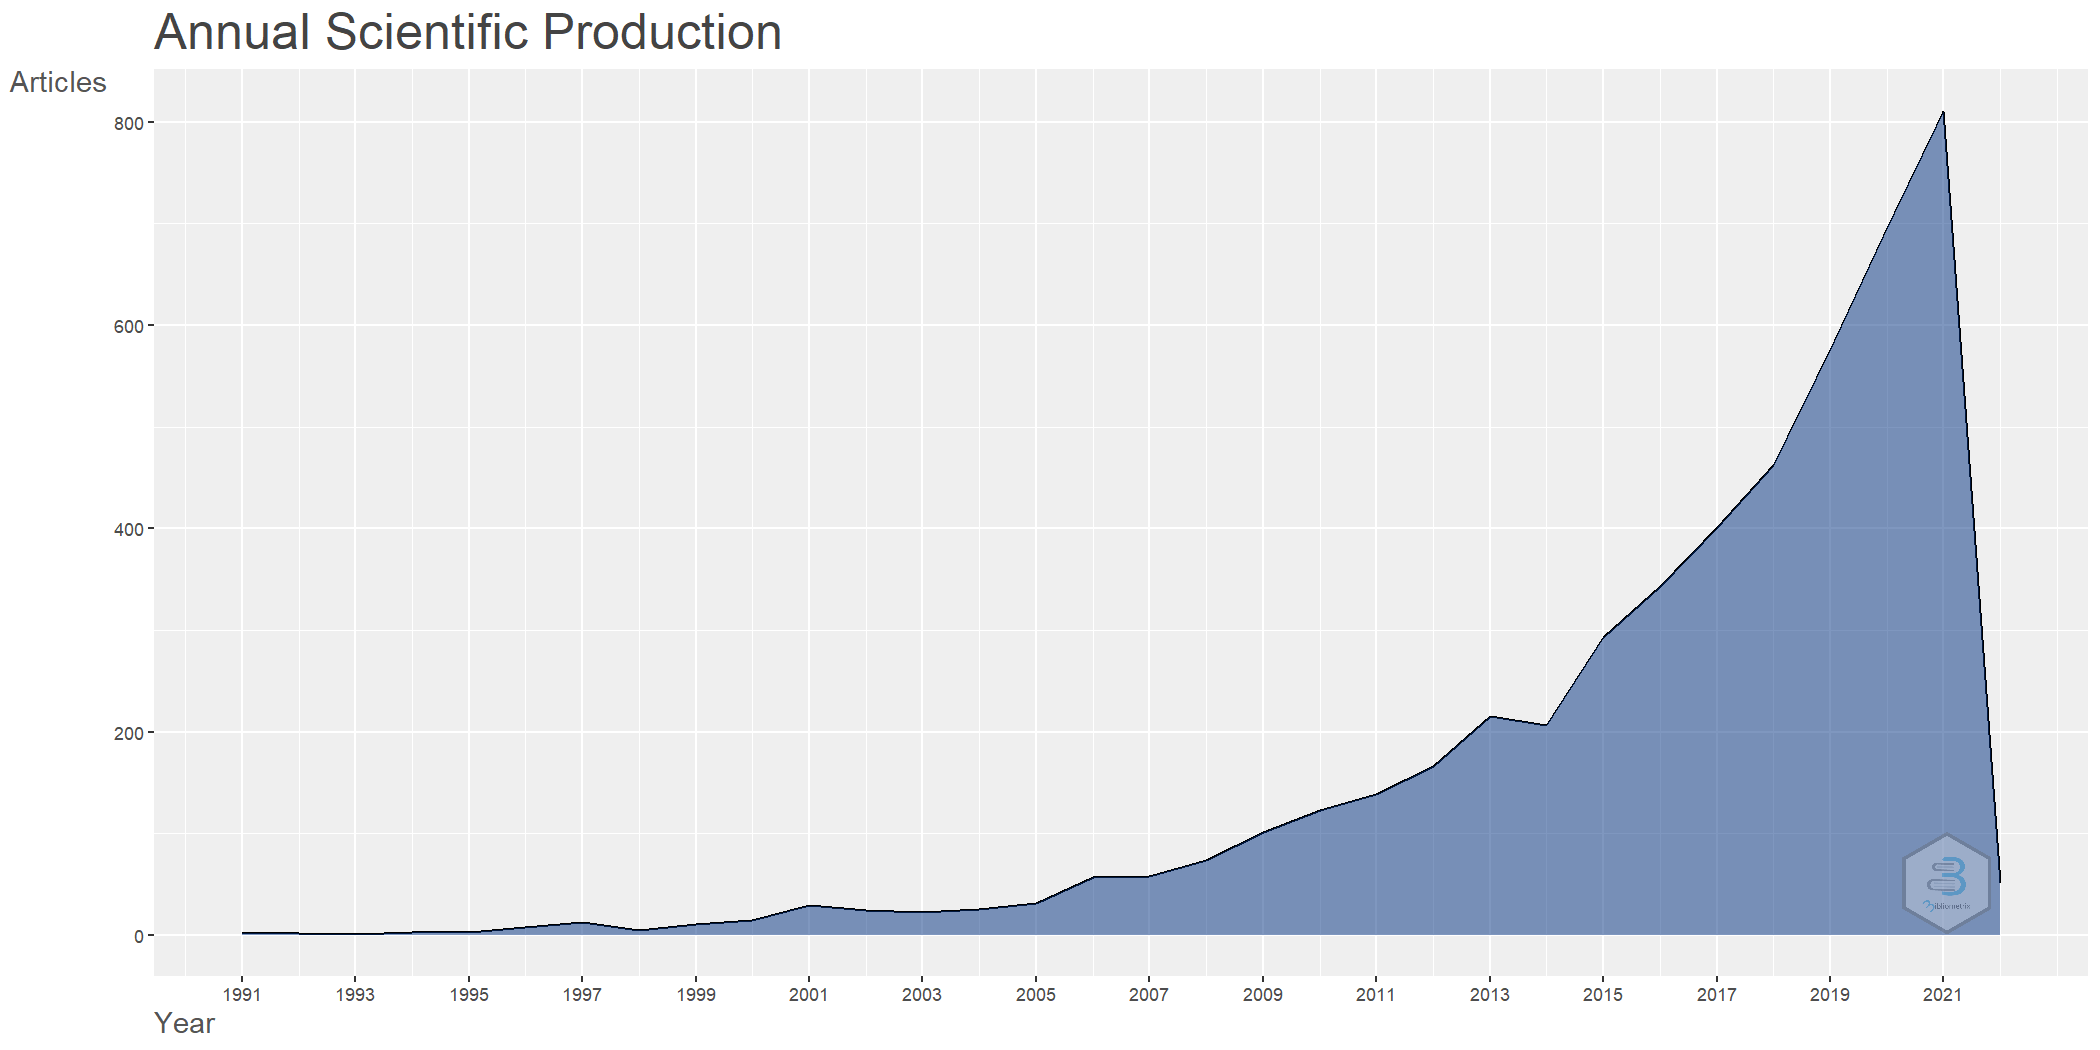
\includegraphics[width=1\textwidth]{experiments/vinis-caixe/PesqBibliogr/MineracaoDados/WoS-20220204/Dataset/AnnualScientificProduction-2022-02-06.png}
    \caption{Evolução da produção científica no \dataset\ .}
    \label{fig:evol:anual:vinis-caixe}
\end{figure}

O \textit{Annual Growth Rate} do \dataset\ é de 11,01\%, tendo 2021 como ano de maior produção de artigos científicos e 1993 o ano com menor produção.

\subsection{Interpretação do Crescimento}

A alta taxa de crescimento indica que existe interesse em utilizar mineração de dados na área de saúde. O fato dos anos 2020 e 2021 terem a maior produção de artigos científicos sugere que o surgimento do coronavírus causou um aumento na pesquisa.

\subsection{Evolução das Citações}

\begin{figure}
    \centering
    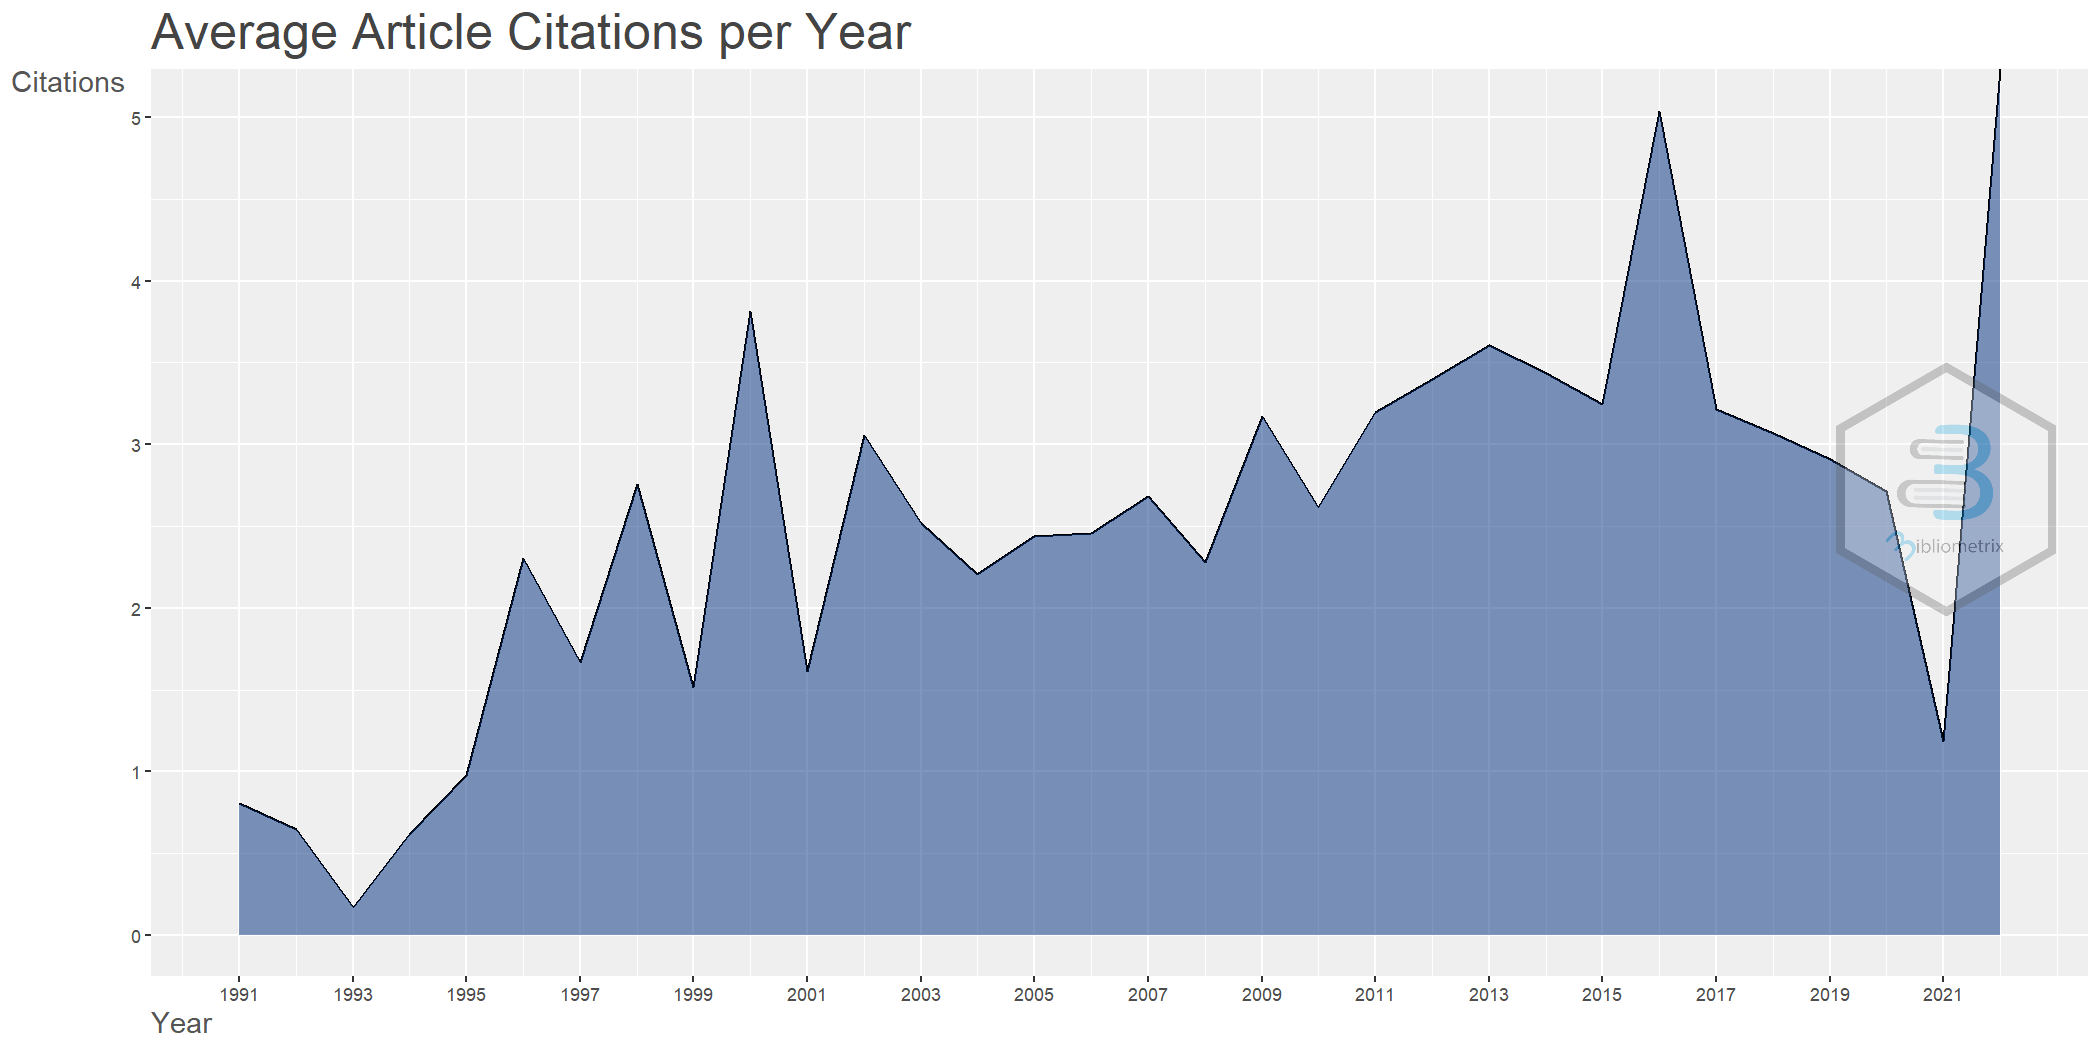
\includegraphics[width=1\textwidth]{experiments/vinis-caixe/PesqBibliogr/MineracaoDados/WoS-20220204/Dataset/AverageArticleCitationPerYear-2022-02-08.png}
    \caption{Média de citações por ano do \dataset\ .}
    \label{fig:cit:anual:vinis-caixe}
\end{figure}